\documentclass[conference]{IEEEtran}
\usepackage{amsmath,booktabs,graphicx,capt-of}
\title{Comparing Attention-Pooled Recurrent Networks for IMDb Sentiment Classification}
\author{\IEEEauthorblockN{Nicholas Ampimah}
\IEEEauthorblockA{University of Nebraska--Lincoln}}
\begin{document}
\maketitle
\begin{abstract}
We compare bidirectional gated recurrent unit (BiGRU) and long short-term memory (BiLSTM) encoders for binary sentiment classification of IMDb reviews. Both use masked attention pooling and classifier dropout of 0.20 or 0.50. A stratified split of the official training set is used for early stopping and model selection. BiLSTM-A, selected by validation cross-entropy, achieved 84.84\% accuracy and 15.16\% error (95\% Wilson CI: 14.72--15.61\%) on 25,000 held-out reviews. Increasing dropout from 0.20 to 0.50 worsened minimum validation loss in both encoders and did not prevent overfitting.
\end{abstract}
\begin{IEEEkeywords}
sentiment analysis, IMDb, recurrent networks, attention, dropout
\end{IEEEkeywords}
\section{Introduction}
Review sentiment depends on word order and context. Negation can reverse the meaning of a phrase, and a later clause can reverse the tone of an earlier one. On IMDb \cite{maas}, we compare BiGRU and BiLSTM encoders with the same attention and classifier layers. Within each architecture we change only dropout to examine whether stronger regularization improves validation performance and changes the training--validation gap. BiLSTM-A was selected at validation loss 0.3027 and achieved 84.84\% test accuracy and 0.848 macro-F1. The four test accuracies spanned only 0.31 percentage points, while all four learning curves showed overfitting after their best checkpoint.

\section{Problem and Data}
The input is a review represented by up to 200 token IDs; $y\in\{0,1\}$ denotes negative or positive sentiment. The model returns $p_\theta(y=1\mid x)$; a score above 0.5 predicts positive. Training minimizes binary cross-entropy,
\begin{equation}
-\frac{1}{B}\sum_{i=1}^{B}[y_i\log p_i+(1-y_i)\log(1-p_i)].
\end{equation}
This objective penalizes confident errors. The fixed threshold avoids test-set threshold tuning.

TensorFlow Datasets supplies 25,000 labeled training and 25,000 test reviews. A seed-42 stratified split gives 20,000 training and 5,000 validation reviews. The official test split remains separate. Lowercasing and removing HTML line breaks and most punctuation reduce vocabulary fragmentation; apostrophes are kept for contractions. The vocabulary contains up to 15,000 entries, including padding and unknown tokens, and is fitted only on training reviews. Padding or truncation to 200 tokens bounds computation, but truncation can discard sentiment evidence late in a review.

\section{Architectures and Training}
A learned embedding maps each token to 64 features. Bidirectional recurrence encodes left and right context because the complete review is available at inference. GRUs use update and reset gates; LSTMs use input, forget, and output gates and a separate cell state. Both use sigmoid gates and tanh state or candidate activations.

\begin{table}[!ht]
\caption{Architecture comparison. Shapes omit the batch dimension.}
\label{tab:architecture}
\centering\footnotesize
\begin{tabular}{@{}lll@{}}
\toprule
Stage & BiGRU & BiLSTM\\
\midrule
Token IDs & 200 & 200\\
Embedding & $200\times64$ & $200\times64$\\
Encoder & GRU, 48/direction & LSTM, 48/direction\\
Encoder output & $200\times96$ & $200\times96$\\
Pooling & Masked attention, 96 & Same\\
Classifier & Dense 32, ReLU, dropout & Same\\
Output & Dense 1, sigmoid & Same\\
Parameters & 999,105 & 1,009,665\\
\bottomrule
\end{tabular}
\end{table}

The attention layer in Table~\ref{tab:architecture} computes $s_t=v^\top\tanh(Wh_t+b)$ using a 32-unit projection, applies softmax over nonpadding tokens, and sums the states $h_t$ weighted by their attention scores after softmax. It can emphasize informative positions throughout the retained text without relying on the final recurrent state. Dropout follows the dense ReLU layer and discourages reliance on individual features. Setting A uses dropout 0.20 and setting B uses 0.50. Both use Adam at $10^{-3}$ and batch size 128.

Training retains the minimum-validation-loss checkpoint, with a patience of five full epochs without improvement. A run that reaches the epoch cap before completing the required window is rejected. The 300-epoch cap was never reached; all four models stopped after five epochs without improvement. The winner was fixed before scoring the official test split. All four frozen checkpoints are evaluated for comparison.

\twocolumn[{
\begin{minipage}{\textwidth}
\centering
\captionof{table}{Held-out performance. Validation loss is measured at the best checkpoint. $^\ast$Selected by validation loss. Error CIs are 95\% Wilson intervals.}
\label{tab:results}
\small
\begin{tabular}{lrrrrrrr}
\toprule
Model & Best / stop & Val. loss & Accuracy (\%) & Macro-F1 & ROC AUC & Error (\%) & Error CI (\%)\\
\midrule
BiGRU-A & 2/7 & 0.3040 & 85.06 & 0.850 & 0.931 & 14.94 & [14.51, 15.39]\\
BiGRU-B & 2/7 & 0.3055 & 85.10 & 0.851 & 0.930 & 14.90 & [14.47, 15.35]\\
BiLSTM-A$^\ast$ & 2/7 & 0.3027 & 84.84 & 0.848 & 0.930 & 15.16 & [14.72, 15.61]\\
BiLSTM-B & 1/6 & 0.3179 & 85.15 & 0.851 & 0.930 & 14.85 & [14.41, 15.29]\\
\bottomrule
\end{tabular}
\end{minipage}\vspace{10pt}

\begin{minipage}{\textwidth}
\centering
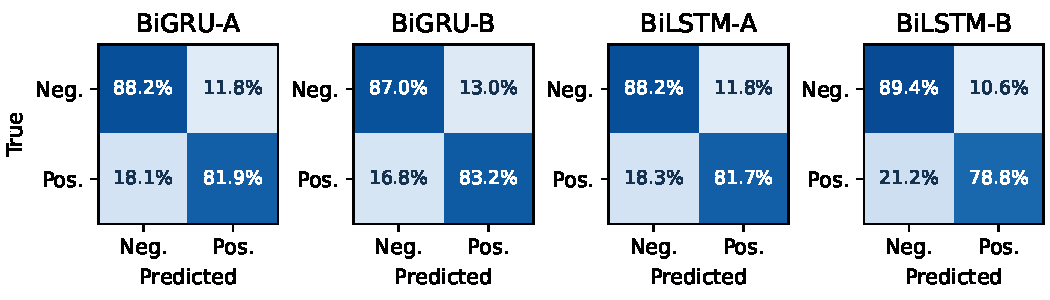
\includegraphics[width=.98\textwidth]{results/confusion_matrices.pdf}
\captionof{figure}{Row-normalized test confusion matrices. Rows are true classes, columns are predicted classes, and diagonal values are class recalls.}
\label{fig:cm}
\end{minipage}\vspace{14pt}
}]
\section{Held-Out Results}
\subsection{Metrics and confidence intervals}
Accuracy summarizes correct classifications, macro-F1 weights both classes equally, and ROC AUC assesses ranking across thresholds. For $k$ errors among $n$ test reviews, the observed error is $\hat e=k/n=1-\mathrm{accuracy}$. Its Wilson interval is
\begin{equation}
\frac{\hat e+z^2/(2n)\ \pm\ z\sqrt{\hat e(1-\hat e)/n+z^2/(4n^2)}}{1+z^2/n},
\end{equation}
where $z=1.96$. The interval describes approximate test-sample uncertainty conditional on the fitted model. It does not measure retraining variability, performance under dataset shift, or paired differences between models evaluated on the same reviews.


\newpage
\subsection{Model selection}
BiLSTM-A had the lowest validation loss (0.3027), narrowly ahead of BiGRU-A (0.3040). BiLSTM-B had the highest observed test accuracy (85.15\%), but its validation loss was worse (0.3179). Accuracy counts decisions at one threshold; cross-entropy also penalizes misplaced confidence. The test ranking is descriptive and does not override validation-based selection. The individual intervals do not establish whether paired differences are statistically meaningful.

\subsection{Class-specific performance}
Figure~\ref{fig:cm} shows the fraction of each true class assigned to each predicted class. False positives are negative reviews predicted positive; false negatives are positive reviews predicted negative. Every model missed more positive reviews than negative ones. BiLSTM-A made 2,327 false negatives versus 1,462 false positives, yielding 81.38\% positive recall and 88.30\% negative recall. With balanced classes, overall accuracy equals the average of the two class recalls.

\twocolumn[{
\begin{minipage}{\textwidth}
\centering
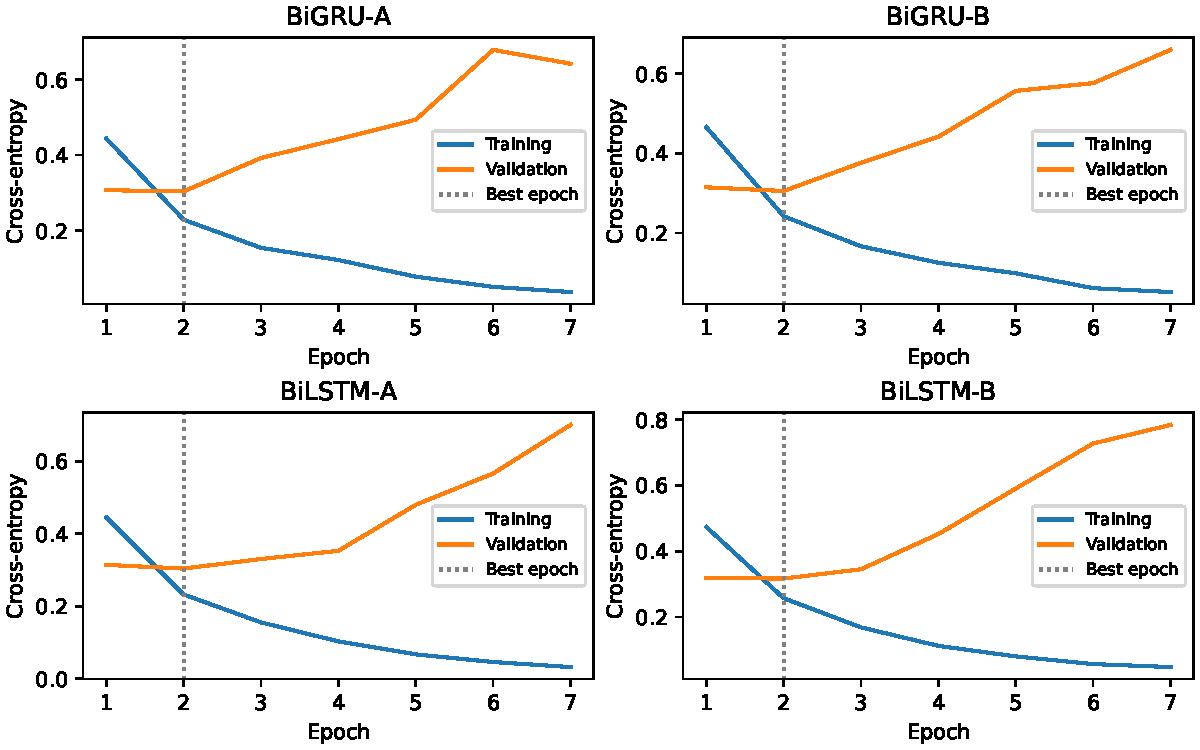
\includegraphics[width=.84\textwidth]{results/learning_curves.pdf}
\captionof{figure}{Binary cross-entropy by epoch. Vertical lines mark the best validation checkpoint for each model.}
\label{fig:curves}
\end{minipage}\vspace{12pt}
}]
\section{Dropout and Overfitting}
For each architecture, compare B minus A in minimum validation loss and in the validation minus training loss at each best epoch. A negative validation-loss change favors stronger dropout. A smaller gap alone is insufficient evidence of better generalization because dropout is active when training loss is measured. The curves in Fig.~\ref{fig:curves} provide a second diagnostic: falling training loss accompanied by rising validation loss suggests overfitting. Early stopping retains the checkpoint before any subsequent validation deterioration.

Increasing dropout changed minimum validation loss from 0.3040 to 0.3055 for BiGRU and from 0.3027 to 0.3179 for BiLSTM. For BiGRU the best-epoch loss gap narrowed from 0.0750 to 0.0635, yet validation loss increased. BiLSTM-B reached its minimum at epoch 1, so its training--validation gap is not directly comparable with BiLSTM-A at epoch 2. All four models continued to reduce training loss after their best epoch while validation loss ultimately rose. For BiLSTM-A, training loss fell from 0.2333 to 0.0331 between epochs 2 and 7, while validation loss rose from 0.3027 to 0.6572. Thus stronger dropout did not eliminate overfitting, and the saved early checkpoint mattered.


\newpage
\section{Strengths and Limitations}
The shared prediction head, identical split, and one-factor dropout comparison support comparisons under a common protocol. Masked attention excludes padding, but its weights do not establish causal explanations. The encoders have different parameter counts, so a difference cannot be attributed to gate design alone. One split and seed limit reproducibility claims. Truncation and the vocabulary cap trade coverage for tractable training. Results apply to polarized movie reviews and do not establish performance on neutral reviews or other domains.

\section{Conclusion}
BiLSTM-A was the validation-selected model and achieved 84.84\% test accuracy, with a 95\% error interval of [14.72, 15.61]\%. No configuration avoided overfitting. Within this single-seed experiment, 0.50 dropout did not improve minimum validation loss for either recurrent cell.

\begin{thebibliography}{1}
\bibitem{maas} A.~L. Maas \emph{et al.}, Learning word vectors for sentiment analysis, in \emph{Proc. ACL-HLT}, 2011, pp. 142--150.
\end{thebibliography}
\end{document}
